


\begin{equation}
x = \frac{-b \pm \sqrt{b^2 - 4ac} }{2a}
\end{equation}

where $x$ is a number; $a$, $b$, and $c$ are other numbers.

\begin{equation}
BCP = 176R+28G+46B
\end{equation}

where, $BCP$, $R$, $G$ and $B$ are also useful numbers.

Figure \ref{fig_regression} shows a graph.  Figures / diagrams / photos are to be centred, with the reference and caption printed below the figure. The lettering used in the illustrations should be easily legible.  Illustrations are to be referred to as figures, and must be quoted in the text. One blank line should be left between the figure caption and the next paragraph. Please ensure that all figures are of the highest quality. Keep figures as simple as possible. Avoid excessive notes. Photographs must have a resolution of at least 300 dpi. The use of colour is allowed on figures. Note that the test does not wrap around the figure but if you do not like the wasted space then it is acceptable to put two figures side by side but they must be e.g. a ‘Figure \ref{fig_bridge1}’ and ‘Figure \ref{fig_bridge2}’ and not ‘Figure 1’ and ‘Figure 2’. See the example given as Figure \ref{fig_twobridges}. However all figures must be as close as possible to the location where they are first referred to in the text. The figure is also not surrounded by an unnecessary box/border. Remove this when inserting figures from MS Excel.


\begin{figure}[ht]
\centering
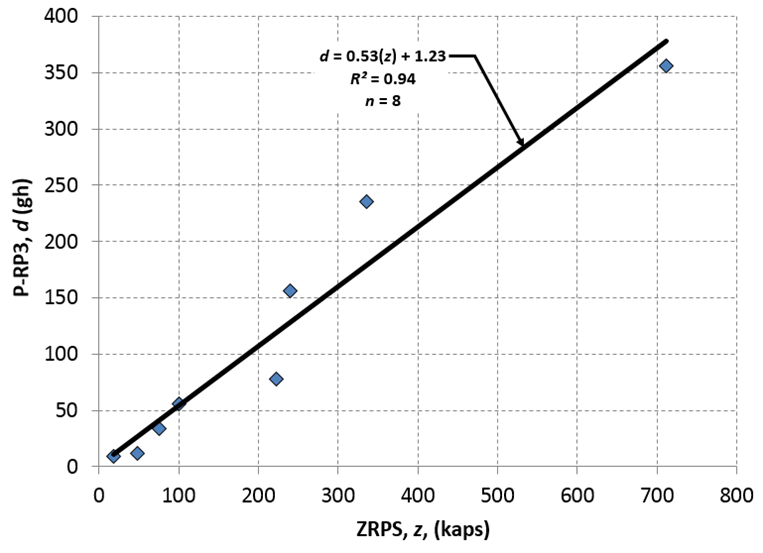
\includegraphics[height=6.6cm]{figures/fig_regression}
\caption{An interesting plot (note that figure captions go BELOW THE FIGURE).}
\label{fig_regression}
\end{figure}


\begin{figure}[ht]
     \centering
     \begin{subfigure}[b]{0.45\textwidth}
         \centering
         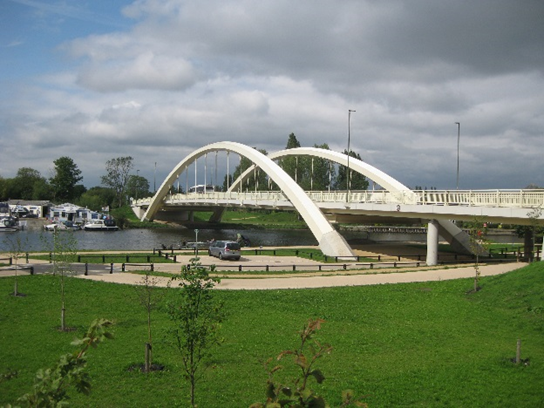
\includegraphics[width=\textwidth]{figures/fig_bridge1}
         \caption{Bridge 1}
         \label{fig_bridge1}
     \end{subfigure}
     \hfill
     \begin{subfigure}[b]{0.45\textwidth}
         \centering
         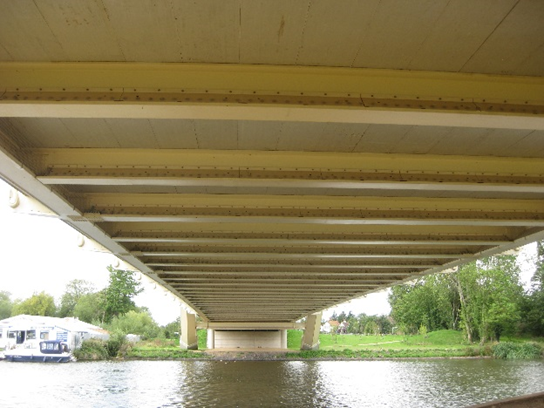
\includegraphics[width=\textwidth]{figures/fig_bridge2}
         \caption{Bridge 2}
         \label{fig_bridge2}
     \end{subfigure}
        \caption{Walton-on-Thames Bridge (a) wide shot and (b) the underside of the deck
(photos taken by P. J. Vardanega, used with permision)}
        \label{fig_twobridges}
\end{figure}